\documentclass{beamer}
\usepackage{graphics}
\usepackage{epsfig}
\usepackage{multicol}
\setbeamertemplate{navigation symbols}{}
\newcommand{\RR}{\ensuremath{\mathbb{R}}}
\newcommand{\NN}{\ensuremath{\mathbb{N}}}
\newcommand{\QQ}{\ensuremath{\mathbb{Q}}}
\newcommand{\CC}{\ensuremath{\mathbb{C}}}
\newcommand{\ZZ}{\ensuremath{\mathbb{Z}}}
\newcommand{\TT}{\ensuremath{\mathbb{T}}}
\DeclareMathOperator{\Min}{Min}
\DeclareMathOperator{\Dom}{Dom}
\DeclareMathOperator{\vol}{vol}
\DeclareMathOperator{\Aut}{Aut}
\DeclareMathOperator{\Stab}{Stab}
\DeclareMathOperator{\Sym}{Sym}
\DeclareMathOperator{\Grp}{Grp}
\DeclareMathOperator{\HYP}{HYP}
\DeclareMathOperator{\CUT}{CUT}
\DeclareMathOperator{\GL}{GL}
\DeclareMathOperator{\AGL}{AGL}
\DeclareMathOperator{\Id}{Id}
\DeclareMathOperator{\vertt}{vert}
\DeclareMathOperator{\conv}{conv}
\DeclareMathOperator{\rank}{rank}

\def\QuotS#1#2{\leavevmode\kern-.0em\raise.2ex\hbox{$#1$}\kern-.1em/\kern-.1em\lower.25ex\hbox{$#2$}}

\begin{document}
\title{Ramanujan $3$-valent plane graphs of positive curvature}
\author{
{\small
\begin{multicols}{2}
\textcolor{red}{\large Mathieu Dutour Sikiri\'c}\\[2mm]
\textcolor{red}{Rudjer Boskovic Institute, Croatia}\\[2mm]
\textcolor{red}{\large Patrick Fowler}\\[2mm]
\textcolor{red}{University of Sheffield, UK}
\end{multicols}
}
}
\date{\today} 
\frame{\titlepage} 





\frame{
\begin{center}
{\Huge 
\begin{tabular*}{6cm}{c}
\\[-0.5cm]
\textcolor{blue}{I. }\textcolor{red}{Ramanujan}\\
\textcolor{red}{graphs}
\end{tabular*}
}
\end{center}
}


\frame{
  \frametitle{Fullerenes}


\begin{itemize}
\item A fullerene is a $3$-valent plane graph, whose faces are $5$ or $6$-gonal.
\item They exist for any even $n\geq 20$, $n\not= 22$.
\begin{center}
%\begin{minipage}[b]{2.3cm}
%\centering
%\resizebox{20mm}{!}{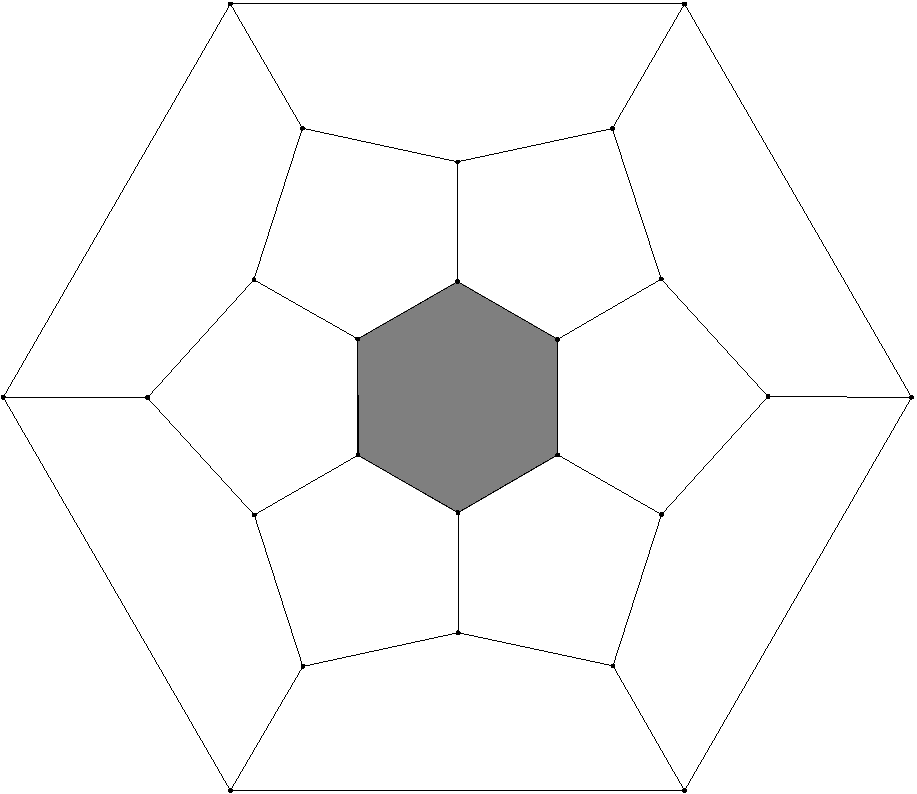
\includegraphics[bb=1 1 440 381, clip]{PictureAppli/F2sec.pdf}}\par
%24
%\end{minipage}
%\begin{minipage}[b]{2.3cm}
%\centering
%\resizebox{20mm}{!}{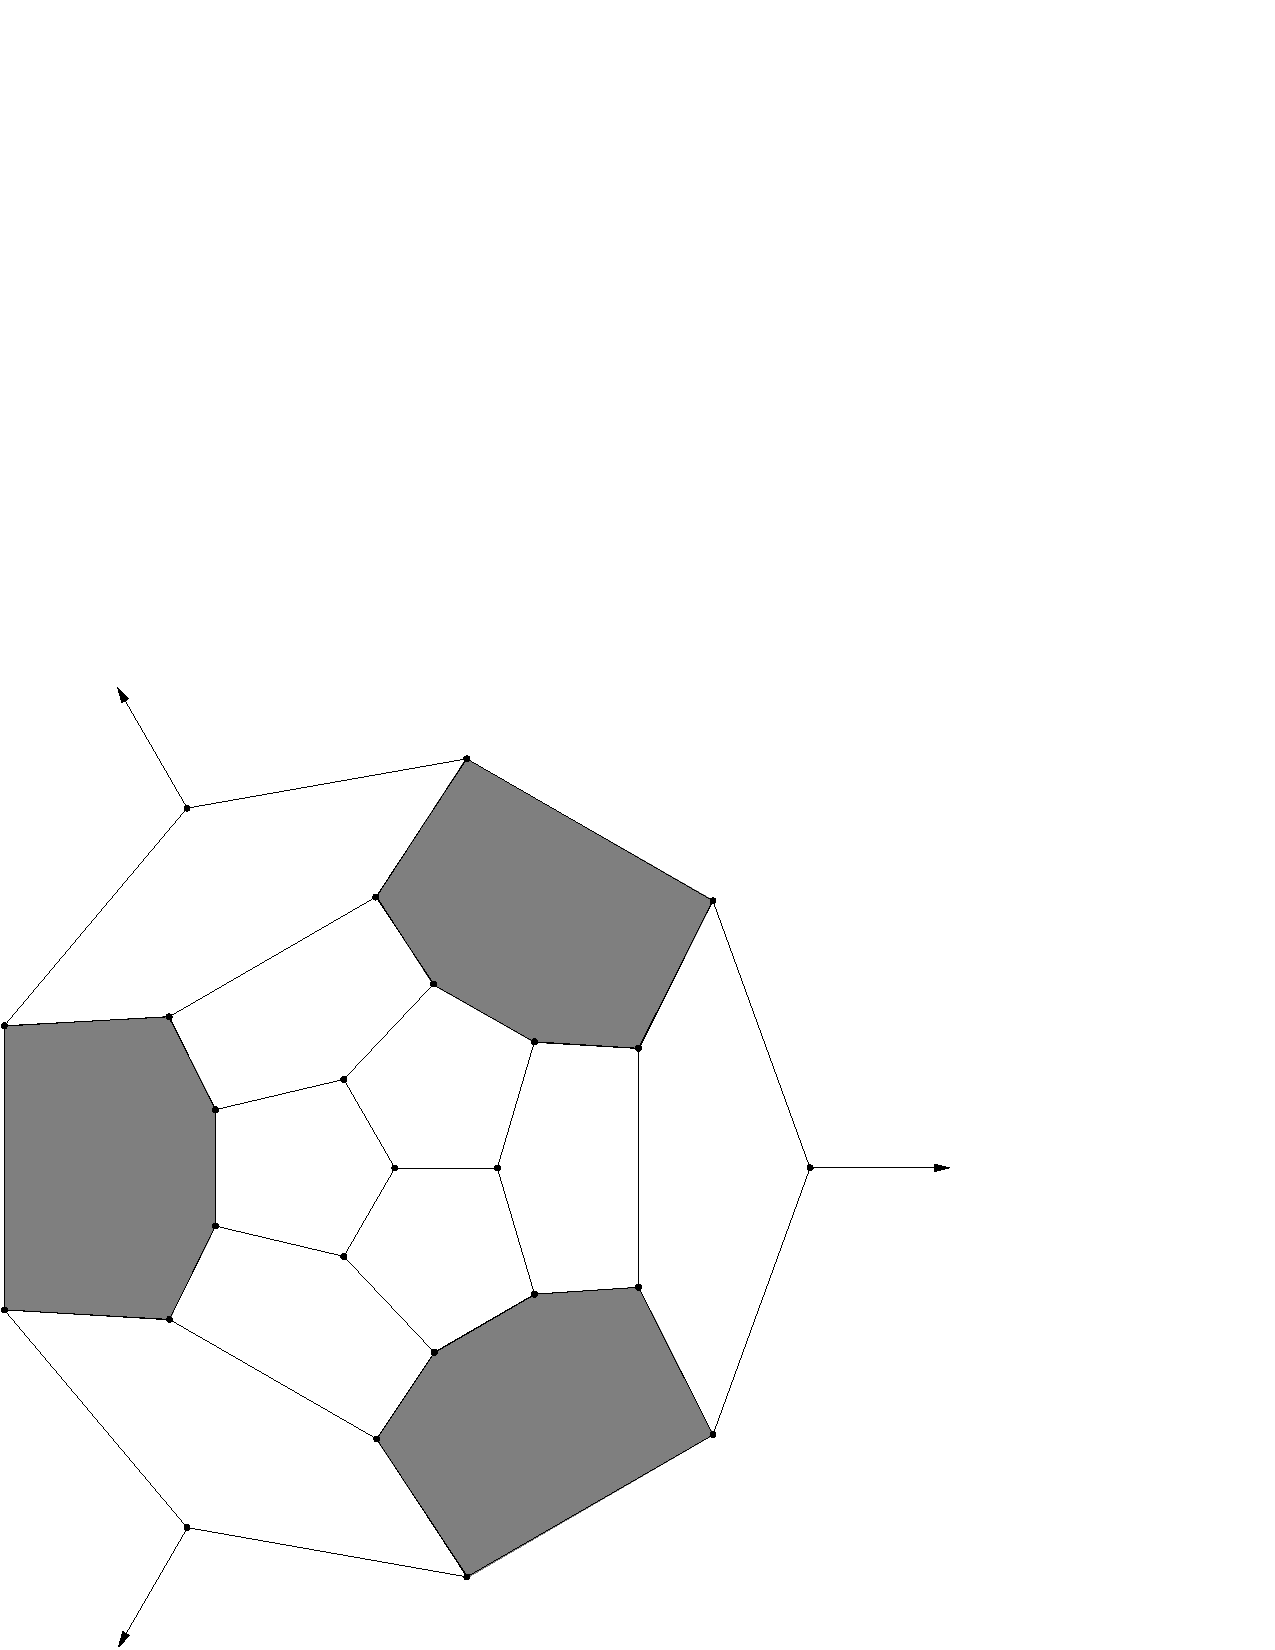
\includegraphics[bb=1 1 457 464, clip]{FullPresPic/Picture2.pdf}}\par
%26
%\end{minipage}
\begin{minipage}[b]{2.3cm}
\centering
\resizebox{13mm}{!}{\rotatebox{90}{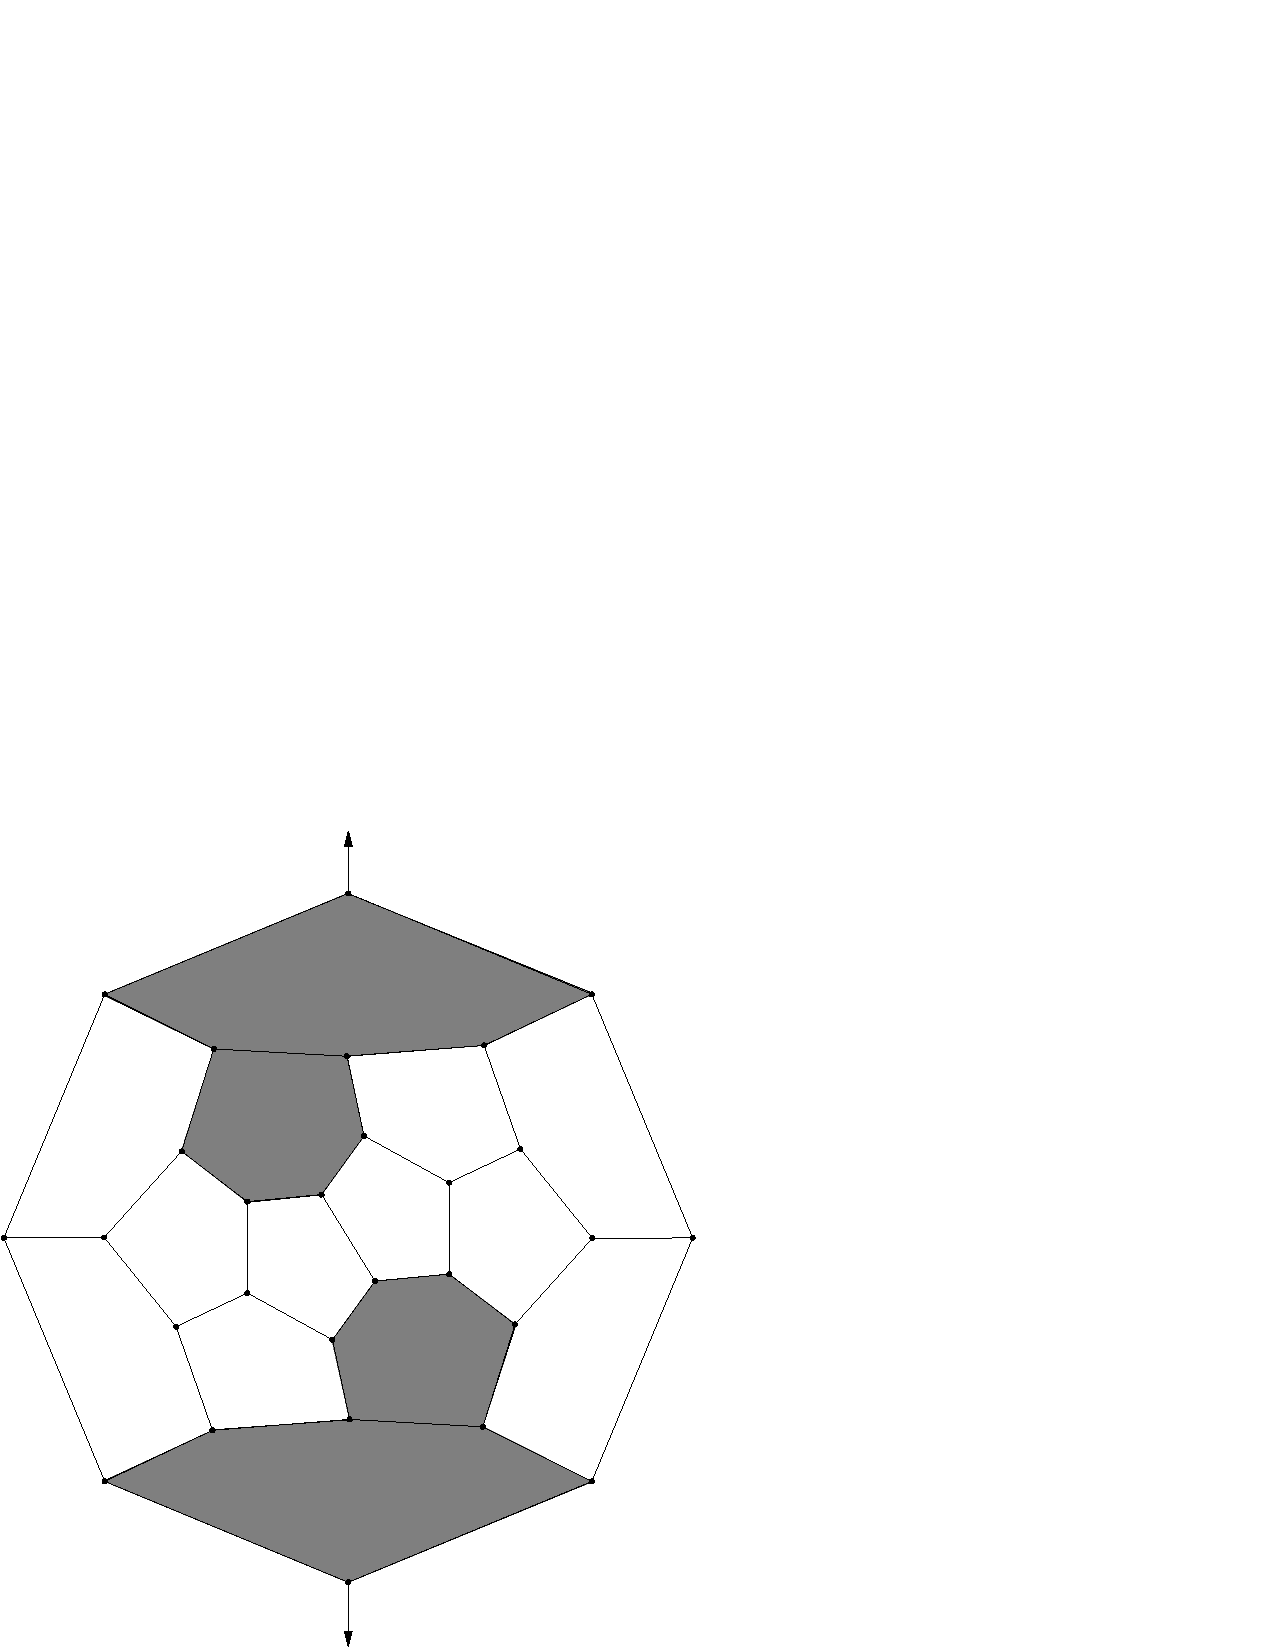
\includegraphics[bb=1 1 333 395, clip]{FullPresPic/Picture3.pdf}}}\par
\end{minipage}
%\begin{minipage}[b]{2.3cm}
%\centering
%\resizebox{20mm}{!}{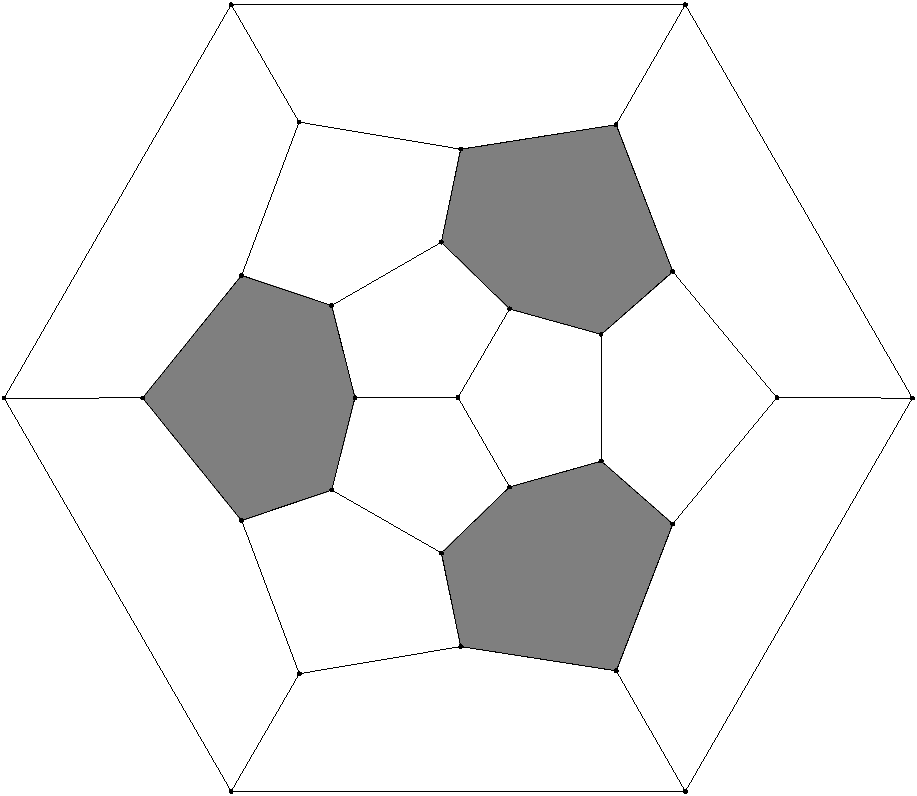
\includegraphics[bb=1 1 439 380, clip]{PictureAppli/F4sec.pdf}}\par
%28
%\end{minipage}
\begin{minipage}[b]{2.3cm}
\centering
\resizebox{11mm}{!}{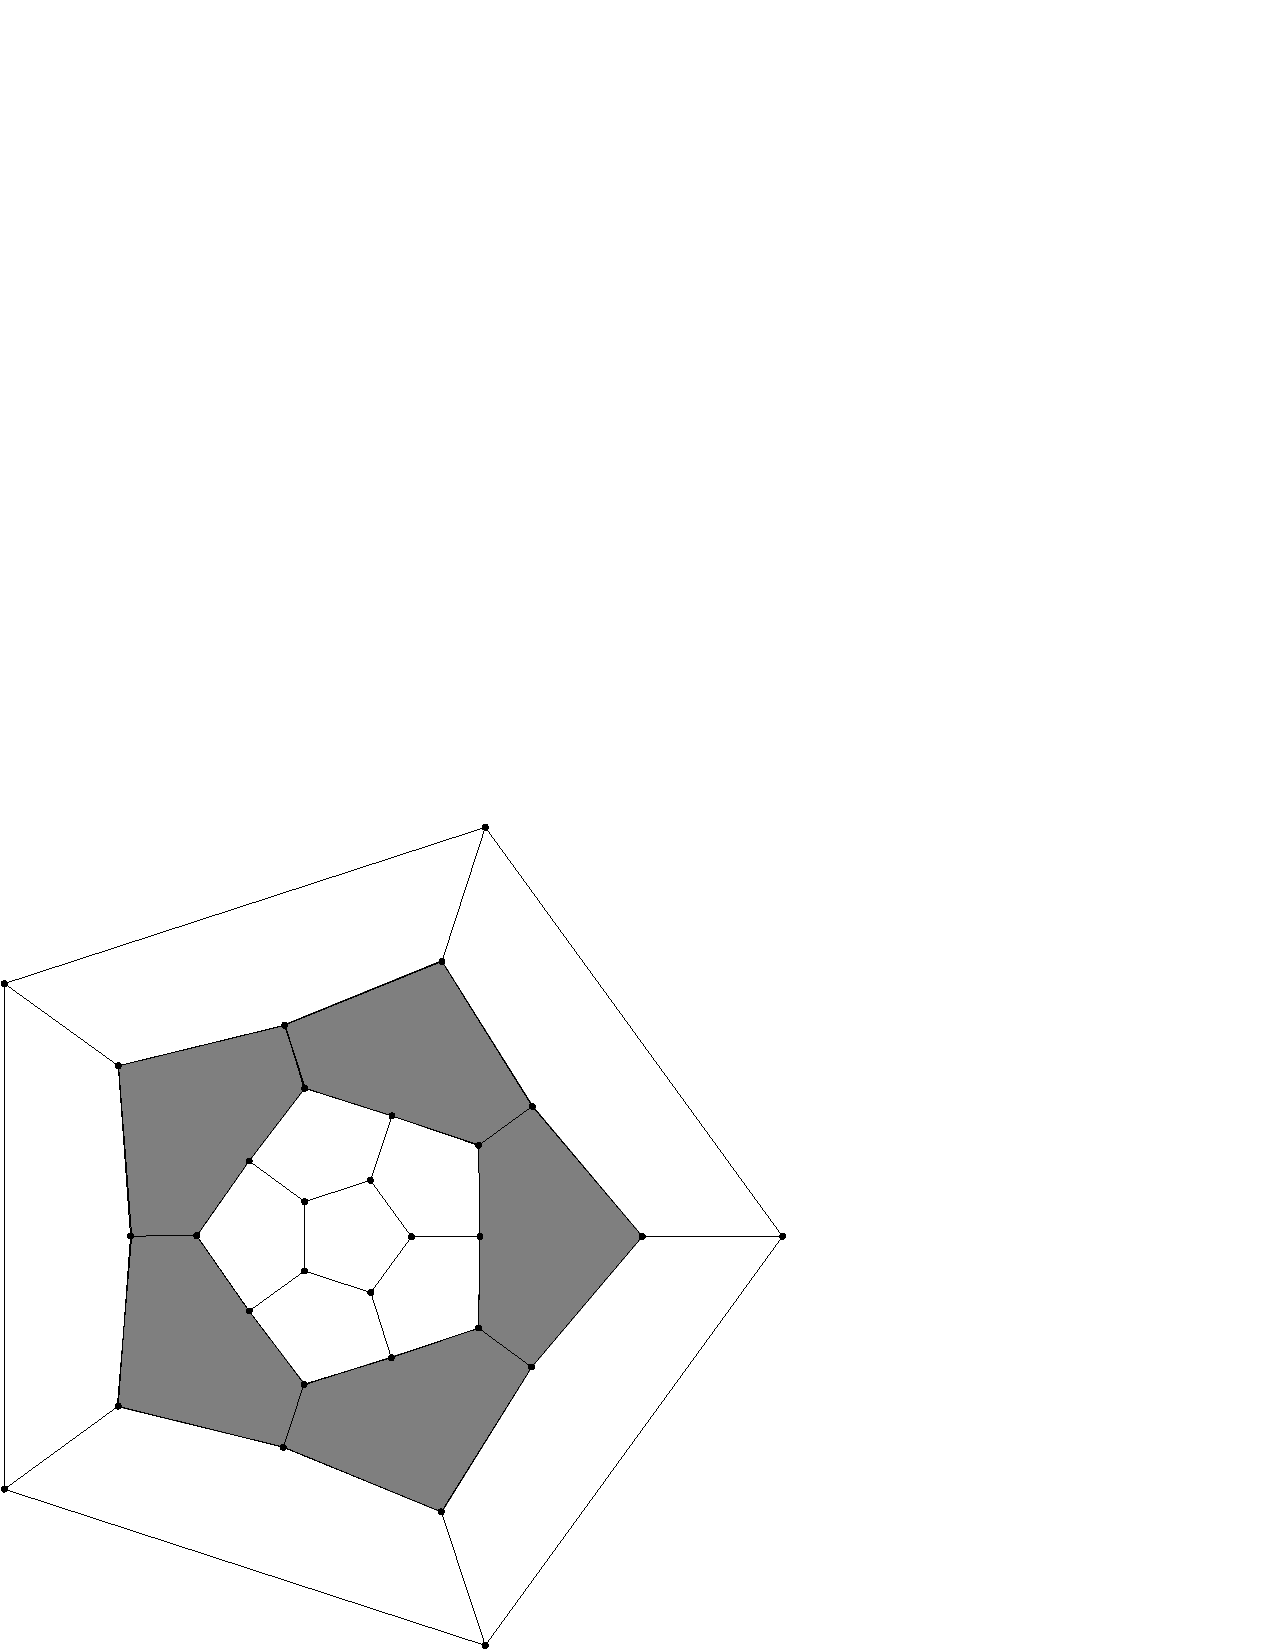
\includegraphics[bb=1 1 377 398, clip]{FullPresPic/Picture5.pdf}}\par
\end{minipage}
\begin{minipage}[b]{2.3cm}
\centering
\resizebox{13mm}{!}{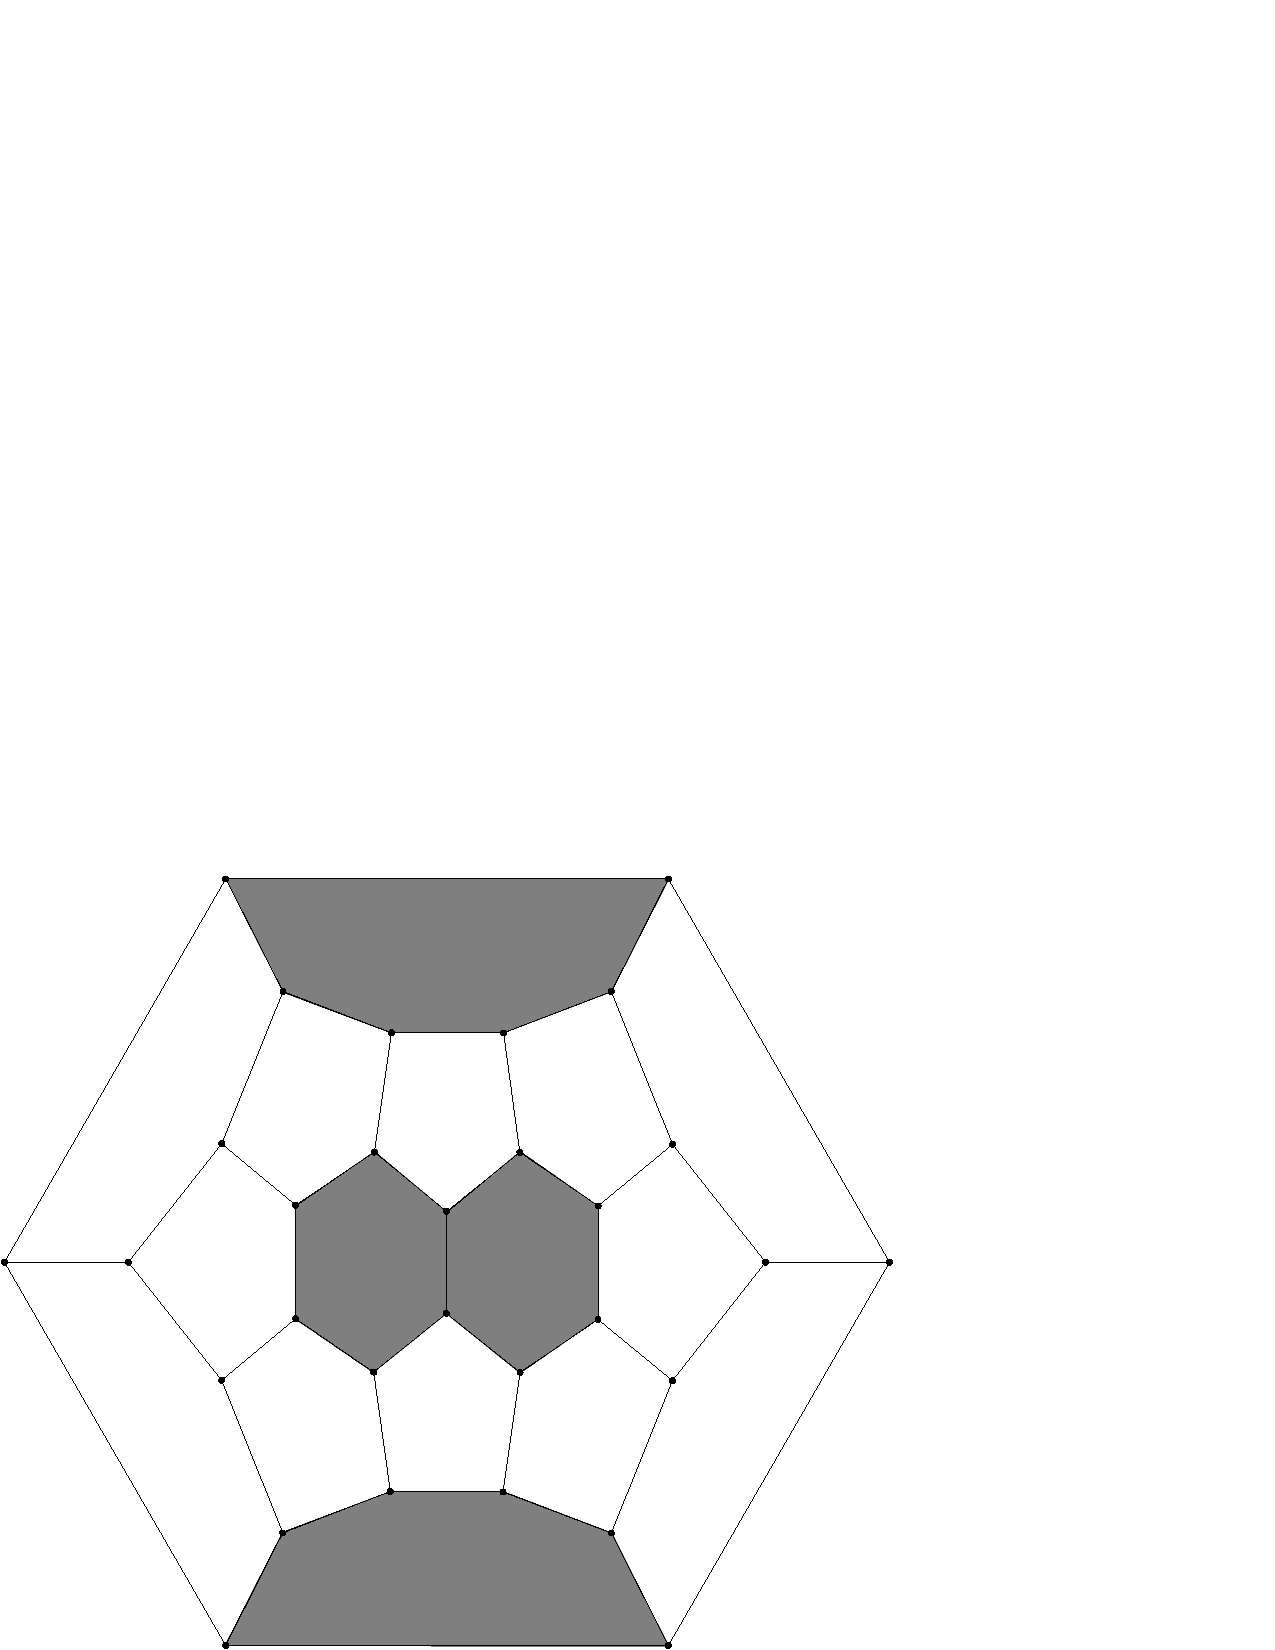
\includegraphics[bb=1 1 429 374, clip]{FullPresPic/Picture6.pdf}}\par
\end{minipage}
\begin{minipage}[b]{2.3cm}
\centering
\resizebox{13mm}{!}{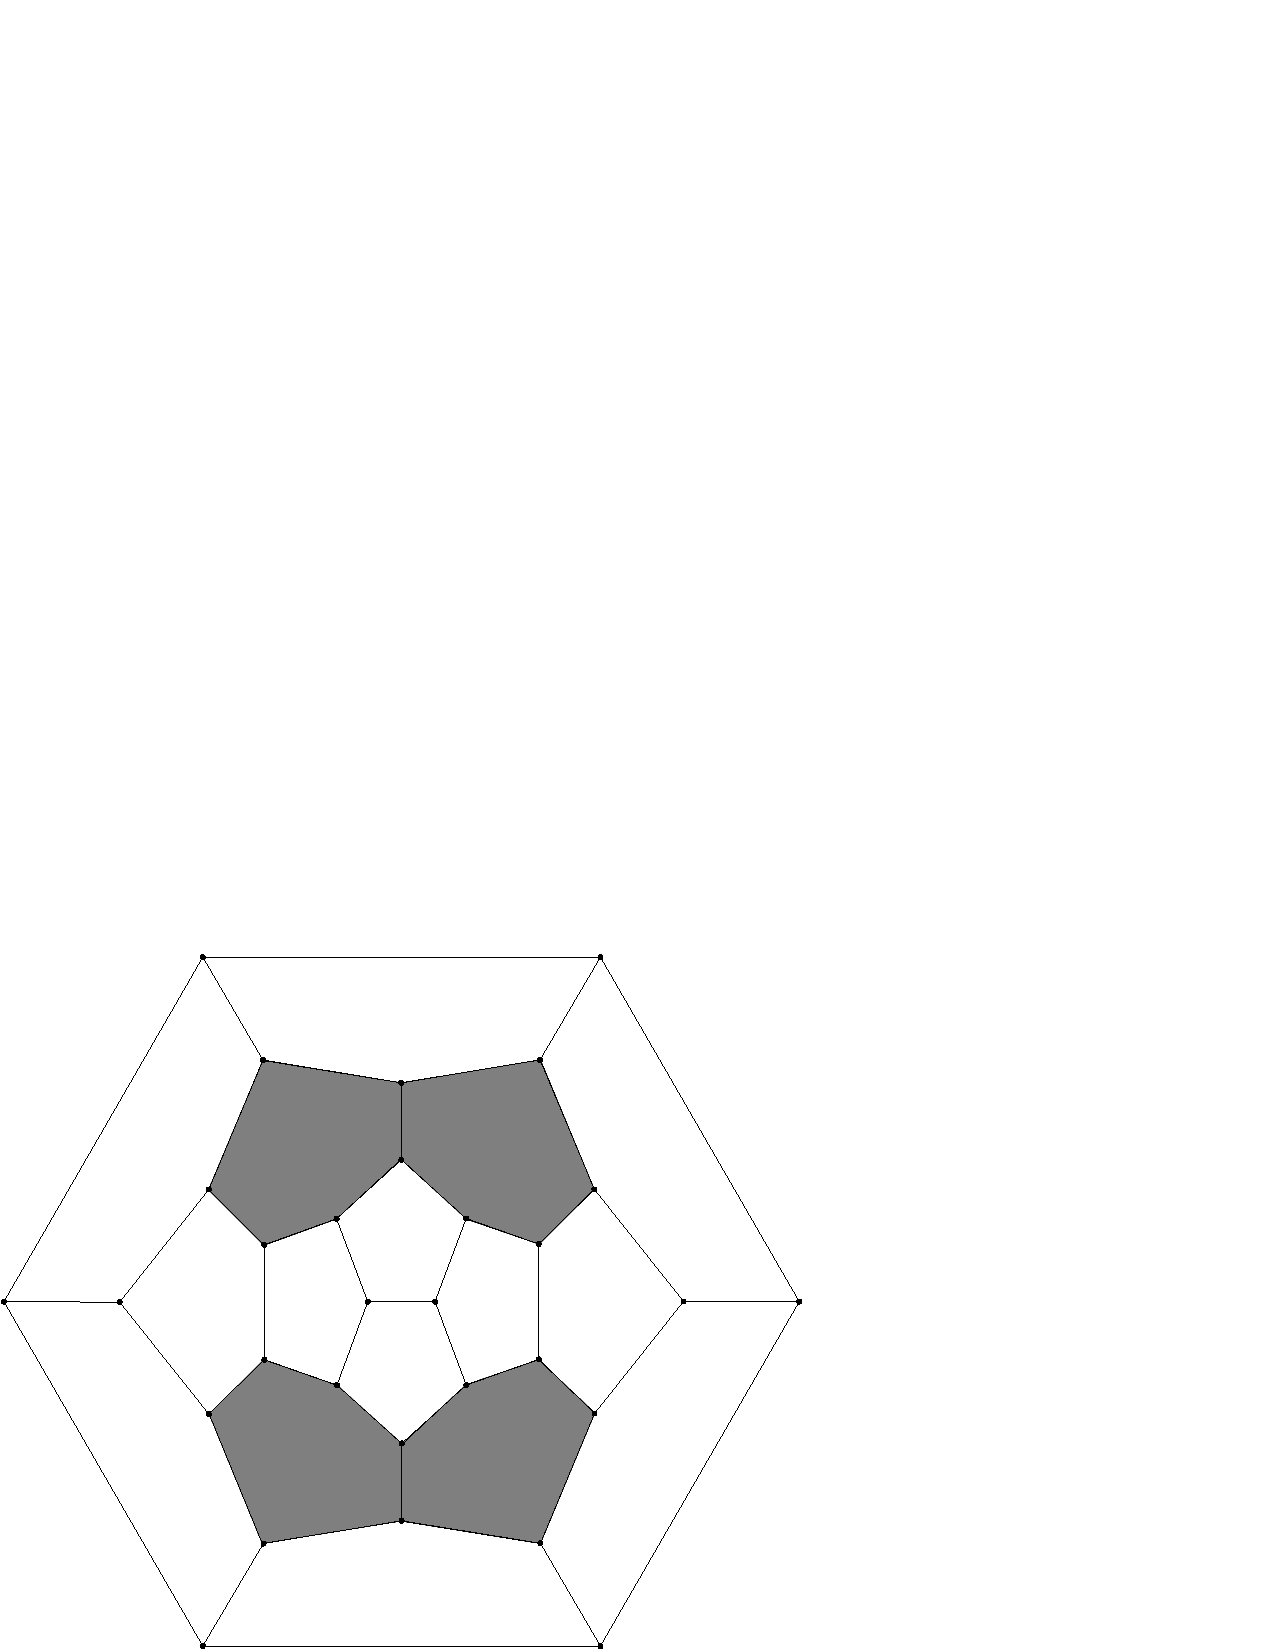
\includegraphics[bb=1 1 385 335, clip]{FullPresPic/Picture7.pdf}}\par
\end{minipage}
\end{center}
\item There exist extremely efficient programs to enumerate them (\textcolor{red}{FullGen} by G. Brinkman, \textcolor{red}{CPF} by T. Harmuth)
\item Fullerenes with isolated pentagons have $n\geq 60$. The smallest one:
\begin{center}
\begin{minipage}{4.5cm}
\centering
\resizebox{30mm}{!}{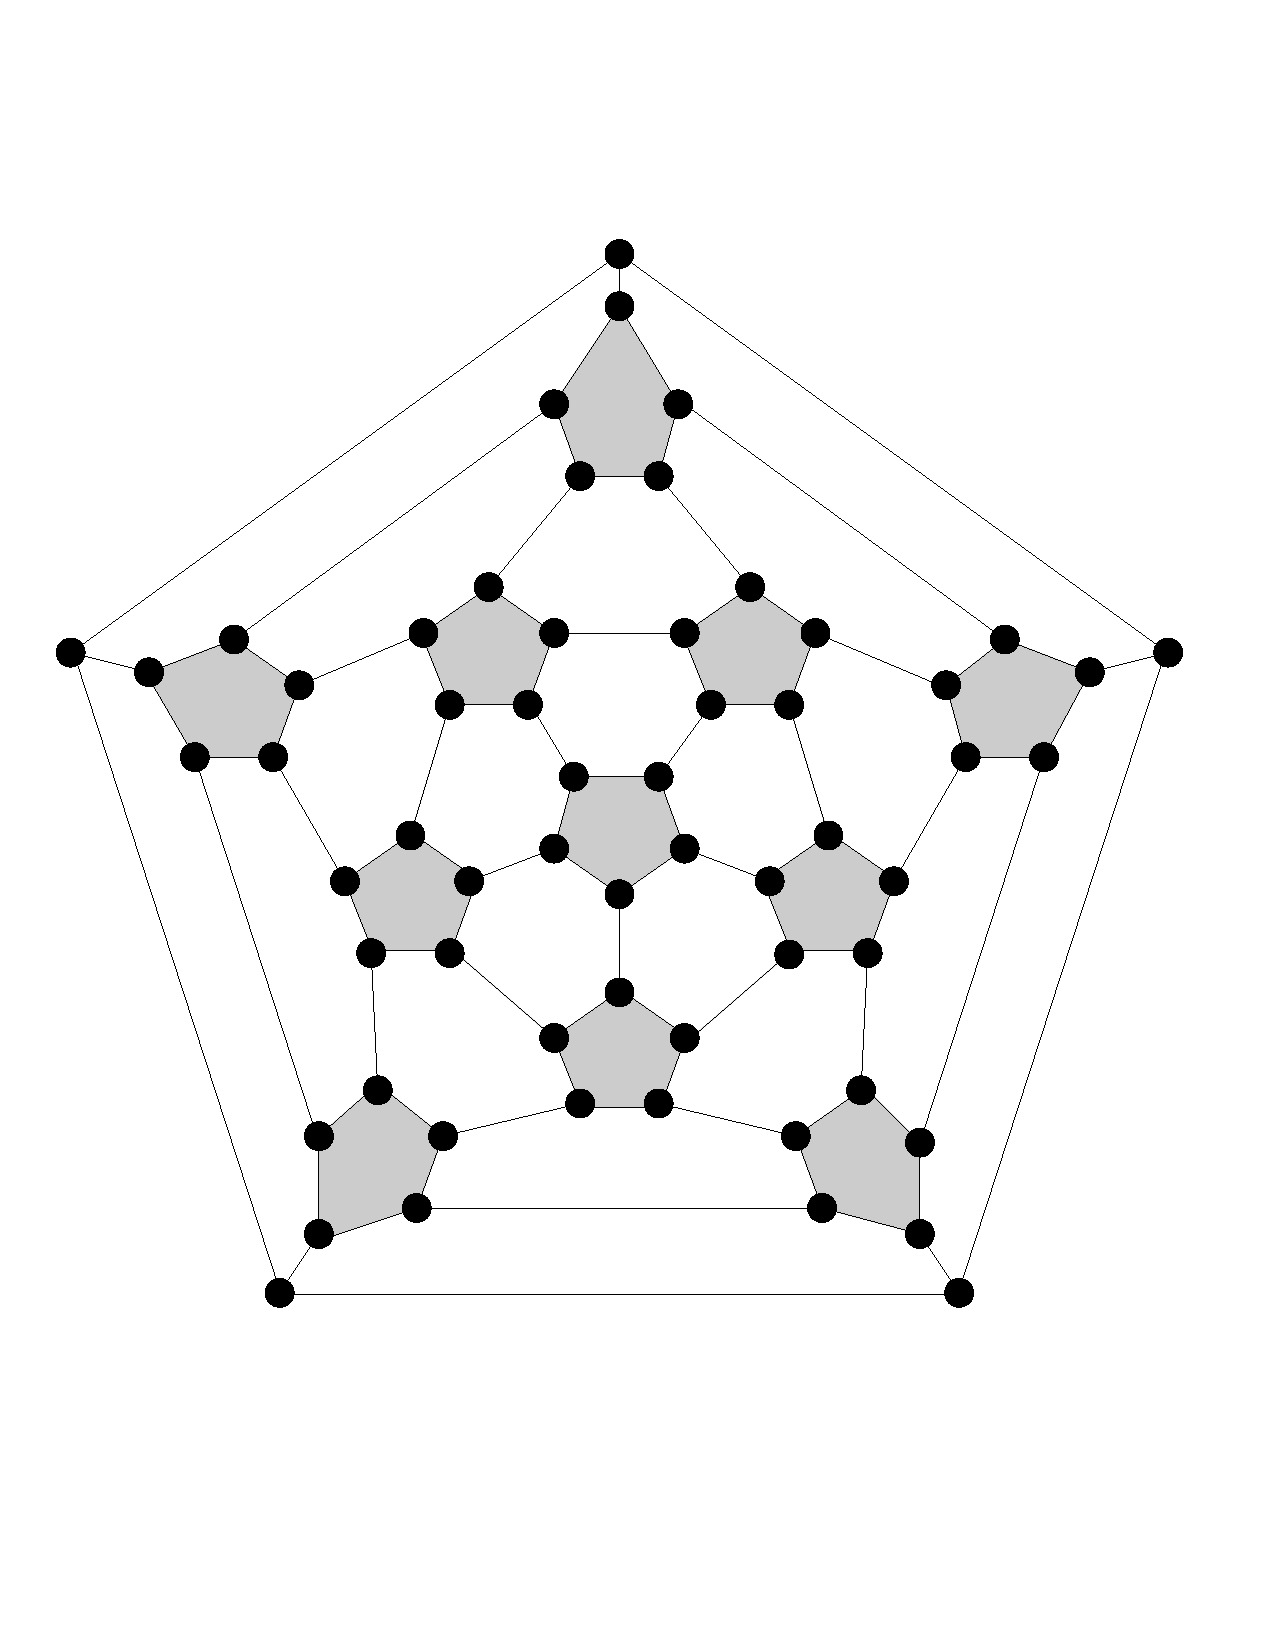
\includegraphics[bb=26 165 568 678, clip]{DRAW/PS/C60.pdf}}\par
\end{minipage}
\begin{minipage}{4.5cm}
\centering
{\em Truncated icosahedron},\par
{\em soccer ball},\par
{\em Buckminsterfullerene}
\end{minipage}


\end{center}
\end{itemize}
}


\frame{
  \frametitle{Graphs of positive curvature}

\begin{itemize}
\item For a $3$-valent plane graph Euler formula can be rewritten as
\begin{equation*}
\sum_{i\geq 3} (6-i) p_i = 12
\end{equation*}
With $p_i$ the number of $i$-gons.
\item Thus it is possible to interpret $6-i$ as the curvature of the face.
\item A $3$-valent plane graph is said to be of \textcolor{red}{positive curvature} if all its face have size between $3$ and $6$.
\item Thus we have the following possibilities for $(p_3, p_4, p_5)$:
\begin{equation*}
\begin{array}{cccc}
(0,0,12) & (0,1,10) & (0,2,8) & (0,3,6)\\
(0,4,4)  & (0,5,2)  & (0,6,0) & (1,0,9)\\
(1,1,7)  & (1,2,5)  & (1,3,3) & (1,4,1)\\
(2,0,6)  & (2,1,4)  & (2,2,2) & (2,3,0)\\
(3,0,3)  & (3,1,1)  & (4,0,0) &
\end{array}
\end{equation*}
\item Such graphs can be very efficiently enumerated with {\tt CPF} by T. Harmuth.
\end{itemize}
}



\frame{
  \frametitle{Eigenvalues and Ramanujan graphs}

\begin{itemize}
\item For a $3$-valent plane graph $G$ the adjacency matrix $A$ is a symmetric matrix with
\begin{itemize}
\item $A(i,j)=1$ if and only if there is an edge between $i$ and $j$.
\end{itemize}
\item $3$ is always an eigenvalue while $-3$ is an eigenvalue if and only if $G$ is bipartite that is has faces of only even size.
\item A $k$-valent graph $G$ is \textcolor{red}{Ramanujan} if all its eigenvalues $\lambda_i$ except $k$ and possibly $-k$ satisfy
\begin{equation*}
|\lambda_i| \leq 2\sqrt{k-1}
\end{equation*}
\item It is called \textcolor{red}{positive Ramanujan}, resp. \textcolor{red}{negative Ramanujan} if the eigenvalues satisfy
\begin{equation*}
\lambda_i \leq 2\sqrt{k-1}\mbox{~~resp.~}\lambda_i \geq -2\sqrt{k-1}
\end{equation*}
Ramanujan graphs are related to expander graphs, which is large subject of research and we are therefore interested which graphs of positive curvature are Ramanujan.
\end{itemize}
}

\frame{
\begin{center}
{\Huge 
\begin{tabular*}{6cm}{c}
\\[-0.5cm]
\textcolor{blue}{I. }\textcolor{red}{Bounds}\\
\textcolor{red}{and strategy}
\end{tabular*}
}
\end{center}
}

\frame{
  \frametitle{The eigenvalue bound}

\begin{itemize}
\item (\textcolor{red}{Alon-Spencer})\textcolor{blue}{Theorem:}
If $G$ is a $k$-regular graph and $\{B, C\}$ is a partition of its vertex
set, then
\begin{equation*}
e(B,C)\geq (k-\lambda_2) \frac{|B|.|C|}{n}
\end{equation*}
with $e(B,C)$ the number of edges between $B$ and $C$ and $\lambda_2$ the second larget eigenvalue.
\item Thus if a graph has a large gap then the separation is large as well.

\end{itemize}
}


\frame{
  \frametitle{Lipton-Tarjan separations}
\begin{itemize}
\item Planar graphs have the property that one can find separations in them.
\item (\textcolor{red}{Lipton-Tarjan}, \textcolor{red}{Alon-Seymour-Thomas}) \textcolor{blue}{Theorem:}
If $G$ is a planar graph then there exists a cycle $F$ of length $n_3$,
that separates $G$ into two patches $P_1$ and $P_2$ with $n_1$ and $n_2$
vertices, satisfying
\begin{equation*}
n_1+\frac{n_3}{2}\leq \frac{2n}{3},\mbox{~~~}
n_2+\frac{n_3}{2}\leq \frac{2n}{3}\quad {\rm and} \quad
n_3\leq 3\frac{\sqrt{2}}{2}\sqrt{n}.
\end{equation*}
\item Thus we can find separation of size proportional to $\sqrt{n}$.
\item Combining both results, we get that if a $3$-valent plane graph is positive Ramanujan then it has at most $875$ vertices.

\end{itemize}
}


\frame{
  \frametitle{Circle packings and Spielman argument}

\begin{itemize}
\item (\textcolor{red}{Spielman-Teng}) \textcolor{blue}{Theorem}: For any plane graph of degree $k$ and $n$ vertices we have
\begin{equation*}
k-\lambda_2 \leq \frac{8k}{n}
\end{equation*}
\item This gives an upper bound of $138$ on positive Ramanujan graphs.
\item Interestingly both this theorem and the previous result of Lipton-Tarjan are proved by associating a Circle Packing to the planar graph.

\end{itemize}
}





\frame{
  \frametitle{General finiteness theorem}

This is only for graphs of positive curvature or for the sake of argument fullerene
\begin{itemize}
\item \textcolor{blue}{Lemma}: If the number $n$ is large enough then a fullerene contains a path of hexagons of large enough size of a nanotube of large enough length.
\item Two proof methods:
\begin{itemize}
\item One is based on a simple covering argument.
\item Another on the theory of parameterization of fullerenes by W. Thurston
\end{itemize}
\item \textcolor{blue}{Theorem:} For any interval $I=[a,b]\subset [-3, 3]$ with $a<b$ the set of fullerenes having no eigenvalue in $I$ is finite.
\item Proof method:
\begin{itemize}
\item The spectrum of the plane tiling by hexagon and of any nanotube is $[-3, 3]$ and each eigenvector is bounded.
\item The rest is easy.
\end{itemize}

\end{itemize}
}

\frame{
  \frametitle{Computational technique}

\begin{itemize}
\item We want to enumerate all Ramanujan graphs.
\item So we enumerate all graphs up to $138$ vertices and check for each of them if they are Ramanujan or not.
\item This gives in practice also the positive Ramanujan as well.
\item For negative Ramanujan, we have only a general non-explicit finiteness result so we do not have complete lists but only some conjectural ones.
\item For computing eigenvalues, we used the Jacobi technique with an estimate of $\epsilon=10^{-5}$.
That is if the eigenvalues satisfy
\begin{equation*}
|\lambda_i| \leq 2\sqrt{2} - \epsilon
\end{equation*}
then they are Ramanujan. If 
\begin{equation*}
|\lambda_i| \geq 2\sqrt{2} + \epsilon \mbox{~for~some~}i
\end{equation*}
then they are not Ramanujan. For the unsolved cases we used Algebraic exact computation, which are much more expensive.


\end{itemize}
}



\frame{
\begin{center}
{\Huge 
\begin{tabular*}{8cm}{c}
\\[-0.5cm]
\textcolor{blue}{II. }\textcolor{red}{Results}\\
\end{tabular*}
}
\end{center}
}



\end{document}
